\section{Experiments}

\subsection{Experimental Setup}
\label{sec:setup}
\paragraph{Datasets and metrics.}
We evaluate CRF-SAM3 on four complementary RVOS benchmarks. \textbf{MeViS}~\cite{ding2023mevis} emphasizes motion expressions and same-category distractors. \textbf{Ref-DAVIS17}~\cite{khoreva2018refdavis} contains short, high-quality videos with language descriptions for multiple objects, while \textbf{Ref-Youtube-VOS}~\cite{seo2020urvos} increases category and scene diversity. \textbf{ReVOS}, introduced with VISA~\cite{yan2024visa}, further includes implicit and reasoning-oriented expressions that may require temporal context and world knowledge. Following standard practice, we report region similarity $\mathcal{J}$, contour accuracy $\mathcal{F}$, and their average $\mathcal{J}\&\mathcal{F}$. For ReVOS we additionally report the official referring and reasoning partitions.

\paragraph{Ground stage.}
The grounder uses Qwen3-VL-4B-Instruct as a frozen backbone. We use $K=8$ target queries of dimension 1024, a two-layer expression conditioner, an $L=2$ query decoder with eight attention heads, a 256-dimensional response head with scale $\gamma=10$, and a modulation adapter with a 512-dimensional bottleneck ($\alpha$ initialized to 0.2). A merged visual token is labelled positive when the target covers at least $\rho=5\%$ of its $2\times2$ merge window. We set $\lambda_g=1.0$ and $\lambda_c=0.5$ and train only the new modules for one epoch in BF16 with gradient checkpointing, a learning rate of $10^{-4}$, 60 warm-up steps, and an effective batch size of 8. Each sample uses $M=3$ frames. During training they are drawn from frames in which the target is annotated, so that $\mathcal{L}_{\mathrm{ground}}$ always receives a non-empty token mask; at inference they are sampled uniformly from the video and resized to a longer side of 336 pixels. The category target $c^{\star}$ is the annotated object category on Ref-Youtube-VOS. ReVOS does not annotate object categories; for its training split, $c^{\star}$ is generated offline as described in the supplementary material. These labels are used only as training targets and are never available at inference. The grounder is trained on the ReVOS training split for ReVOS and on Ref-Youtube-VOS for the other three benchmarks.

\paragraph{Recall and verification.}
SAM3 recall uses SAM3-DMS propagation with $K_r=24$ and $K_{\mathrm{keep}}=7$. The verifier is Qwen3-VL-4B-Instruct with a frozen vision encoder and LoRA ($r=16$, $\alpha=32$, dropout 0.05) on the query, key, value, output, gate, up, and down projections of the language model. Each candidate is represented by $F=4$ frames with a semi-transparent mask overlay, and at most 10 candidates per expression enter a listwise step. We use $\kappa=1$, $\tau_a=1$, $\delta=0.1$, $\lambda_a=0.3$, a learning rate of $10^{-5}$, and one training epoch. The verifier training caches are produced offline by the recall stage of Sec.~\ref{sec:recall}, prompted with training-time concepts (see the supplementary material). A three-domain verifier is first trained jointly on MeViS, Ref-DAVIS17, and Ref-Youtube-VOS (sampling ratio 1:4:2) and is used for these three benchmarks. For ReVOS, it is warm-started from the three-domain checkpoint and further trained on ReVOS. Dataset-specific labelling and ranking settings are listed in Table~\ref{tab:verifier_cfg}. The reported ReVOS number is the \emph{complete validation run}: predictions are produced for all 5,822 validation expressions, and all metrics are taken from the official evaluator outputs.

\begin{table}[t]
\centering
\setlength{\tabcolsep}{4.2pt}
\renewcommand{\arraystretch}{1.08}
\resizebox{\columnwidth}{!}{%
\begin{tabular}{lccccc}
\toprule
Training set & $\theta_{\mathrm{pos}}$ & $\theta_{\mathrm{neg}}$ & Negatives $\mathcal{N}$ & $\lambda_h$ & $r^{+}$ \\
\midrule
MeViS & 0.2 & 0.05 & $J\le\theta_{\mathrm{neg}}$ & 0.15 & mean \\
Ref-DAVIS17 & 0.5 & 0.1 & all non-positive & 0.3 & max \\
Ref-Youtube-VOS & 0.5 & 0.1 & all non-positive & 0.3 & max \\
ReVOS & 0.5 & 0.1 & all non-positive & 0.3 & max \\
\bottomrule
\end{tabular}}
\caption{Verifier labelling and ranking settings per training set.}
\label{tab:verifier_cfg}
\end{table}

\subsection{Benchmark Performance}
\paragraph{Q1: How well does the framework perform across RVOS settings?}
We compare against a compact set of representative methods that are directly related to grounding, foundation video segmentation, MLLM reasoning, or decoupled trajectory selection. The purpose is to position CRF-SAM3 among closely related paradigms rather than to construct an exhaustive leaderboard over rapidly evolving concurrent systems.

\paragraph{Motion-centric evaluation on MeViS.}
MeViS is particularly relevant to our candidate-based formulation because many expressions distinguish objects by motion rather than by category alone. Table~\ref{tab:mevis} keeps the organizer-evaluated val split and the locally evaluable val$^u$ split separate. CRF-SAM3 obtains 68.83 $\mathcal{J}$, 74.07 $\mathcal{F}$, and 71.45 $\mathcal{J}\&\mathcal{F}$ on val$^u$. This result is notable in a benchmark dominated by motion cues and same-category ambiguity, where retaining several plausible object tubes before final discrimination is particularly natural.

\begin{table}[t]
\centering
\setlength{\tabcolsep}{5.4pt}
\renewcommand{\arraystretch}{1.08}
\resizebox{\columnwidth}{!}{%
\begin{tabular}{lcc}
\toprule
Method & MeViS val & MeViS val$^u$ \\
& $\mathcal{J}\&\mathcal{F}$ & $\mathcal{J}\&\mathcal{F}$ \\
\midrule
Sa2VA~\cite{yuan2025sa2va} & 46.9 & 57.1 \\
SAMWISE~\cite{cuttano2024samwise} & 49.5 & 57.1 \\
GLUS~\cite{lin2025glus} & 51.3 & -- \\
VRS-HQ-7B~\cite{gong2025vrshq} & 50.6 & -- \\
\midrule
\textbf{CRF-SAM3 (Ours)} & -- & \textbf{71.45} \\
\bottomrule
\end{tabular}}
\caption{Representative comparison on MeViS. Val and val$^u$ use different evaluation protocols and are therefore shown separately.}
\label{tab:mevis}
\end{table}

\paragraph{Ref-Youtube-VOS and Ref-DAVIS17.}
Table~\ref{tab:standard_rvos} reports the two standard RVOS benchmarks. CRF-SAM3 reaches -- $\mathcal{J}$, -- $\mathcal{F}$, and -- $\mathcal{J}\&\mathcal{F}$ on Ref-Youtube-VOS. On Ref-DAVIS17, it obtains -- $\mathcal{J}$, -- $\mathcal{F}$, and -- $\mathcal{J}\&\mathcal{F}$.

\begin{table*}[t]
\centering
\setlength{\tabcolsep}{5.2pt}
\renewcommand{\arraystretch}{1.08}
\resizebox{0.88\textwidth}{!}{%
\begin{tabular}{ll|ccc|ccc}
\toprule
\multirow{2}{*}{Method} & \multirow{2}{*}{Year}
& \multicolumn{3}{c|}{Ref-Youtube-VOS}
& \multicolumn{3}{c}{Ref-DAVIS17} \\
\cmidrule(lr){3-5}\cmidrule(lr){6-8}
& & $\mathcal{J}$ & $\mathcal{F}$ & $\mathcal{J}\&\mathcal{F}$
& $\mathcal{J}$ & $\mathcal{F}$ & $\mathcal{J}\&\mathcal{F}$ \\
\midrule
SAMWISE~\cite{cuttano2024samwise} & 2025
& 67.8 & 70.6 & 69.2 & 67.4 & 74.5 & 70.6 \\
ReferDINO~\cite{liang2025referdino} & 2025
& 67.0 & 71.5 & 69.3 & 65.1 & 72.9 & 68.9 \\
Sa2VA~\cite{yuan2025sa2va} & 2025
& -- & -- & 70.7 & -- & -- & 75.9 \\
GLUS~\cite{lin2025glus} & 2025
& 65.5 & 69.0 & 67.3 & -- & -- & -- \\
VRS-HQ-7B~\cite{gong2025vrshq} & 2025
& 68.3 & 72.5 & 70.4 & 72.6 & 79.4 & 76.0 \\
DeRVOS~\cite{cheng2026dervos} & 2026
& 68.0 & 71.9 & 70.0 & 68.3 & 73.5 & 70.9 \\
\midrule
\textbf{CRF-SAM3-4B (Ours)} & --
& -- & -- & --
& -- & -- & -- \\
\bottomrule
\end{tabular}}
\caption{Comparison with representative prior work on Ref-Youtube-VOS and Ref-DAVIS17. The table is intended to position CRF-SAM3 among closely related RVOS paradigms rather than provide an exhaustive leaderboard of concurrent systems.}
\label{tab:standard_rvos}
\end{table*}

\paragraph{Full-validation evaluation on ReVOS.}
ReVOS is a useful stress test for our decomposition because the semantics sufficient to recall an object family can be substantially coarser than the semantics required to resolve an implicit or reasoning-heavy expression. Table~\ref{tab:revos_results} reports the official validation metrics from the completed 5,822-expression run. CRF-SAM3 obtains 64.92 $\mathcal{J}\&\mathcal{F}$ on referring expressions, 54.56 on reasoning expressions, and 59.74 overall. The approximately ten-point gap between the two partitions indicates that the final verifier remains substantially more challenged by reasoning-oriented queries than by direct referring expressions.

\begin{table}[t]
\centering
\setlength{\tabcolsep}{3.8pt}
\renewcommand{\arraystretch}{1.08}
\resizebox{\columnwidth}{!}{%
\begin{tabular}{l|ccc}
\toprule
Method & Ref. & Reason. & Overall \\
& \multicolumn{3}{c}{$\mathcal{J}\&\mathcal{F}$} \\
\midrule
VRS-HQ-7B~\cite{gong2025vrshq} & 62.1 & 56.1 & 59.1 \\
VRS-HQ-13B~\cite{gong2025vrshq} & 63.3 & 56.8 & 60.0 \\
Refer-Agent~\cite{jiang2026referagent} & 65.0 & 57.7 & 61.3 \\
\midrule
\textbf{CRF-SAM3-4B (Ours)} & 64.92 & 54.56 & 59.74 \\
\bottomrule
\end{tabular}}
\caption{Representative comparison on the complete ReVOS validation run. Ref. and Reason. denote the official referring and reasoning partitions; Overall is the official evaluator output.}
\label{tab:revos_results}
\end{table}

For completeness, the official CRF-SAM3 ReVOS outputs are $\mathcal{J}=62.51$, $\mathcal{F}=67.34$ for the referring partition, $\mathcal{J}=51.90$, $\mathcal{F}=57.22$ for the reasoning partition, and $\mathcal{J}=57.20$, $\mathcal{F}=62.28$ overall.

\subsection{Candidate-Space and Verification Analysis}
\paragraph{Full-validation ReVOS diagnostic.}
Before turning to controlled training-side diagnostics, we use the score traces saved during the completed ReVOS validation run to inspect the two explicit interfaces exposed by CRF-SAM3: candidate availability after recall and score separation during verification. Among the 3,130 official referring expressions, SAM3 returns no retained candidate for 30 cases (0.96\%); among the 2,475 reasoning expressions, this occurs for 78 cases (3.15\%). These zero-candidate cases obtain only 6.90 and 5.01 mean $\mathcal{J}\&\mathcal{F}$, respectively, illustrating the irreversibility of complete recall failure. Candidate-set cardinality also differs across the two partitions: 76.1\% of referring expressions retain at least two scored hypotheses, compared with 56.8\% of reasoning expressions, while a single retained hypothesis occurs in 22.9\% and 40.0\% of the two partitions.

For expressions with at least two scored candidates, we further compute the verifier score margin $\Delta=s_{(1)}-s_{(2)}$ between the highest- and second-highest-ranked candidates. Figure~\ref{fig:revos_fullval_diag} groups expressions into within-partition margin quartiles. Mean final $\mathcal{J}\&\mathcal{F}$ rises monotonically from 45.13 to 84.27 for referring expressions and from 29.99 to 74.67 for reasoning expressions. The corresponding Spearman correlations between $\Delta$ and final $\mathcal{J}\&\mathcal{F}$ are 0.40 and 0.44, while low-margin cases ($\Delta<0.1$) are more frequent for reasoning expressions (32.5\%) than for referring expressions (20.3\%). We treat this as a post-hoc diagnostic rather than a causal attribution: the score margin reflects both semantic ambiguity and the quality of the recalled hypotheses. Nevertheless, the analysis shows on the full validation run that candidate availability and candidate-level ambiguity are both measurable failure interfaces of the proposed decomposition.

\begin{figure*}[t]
  \centering
  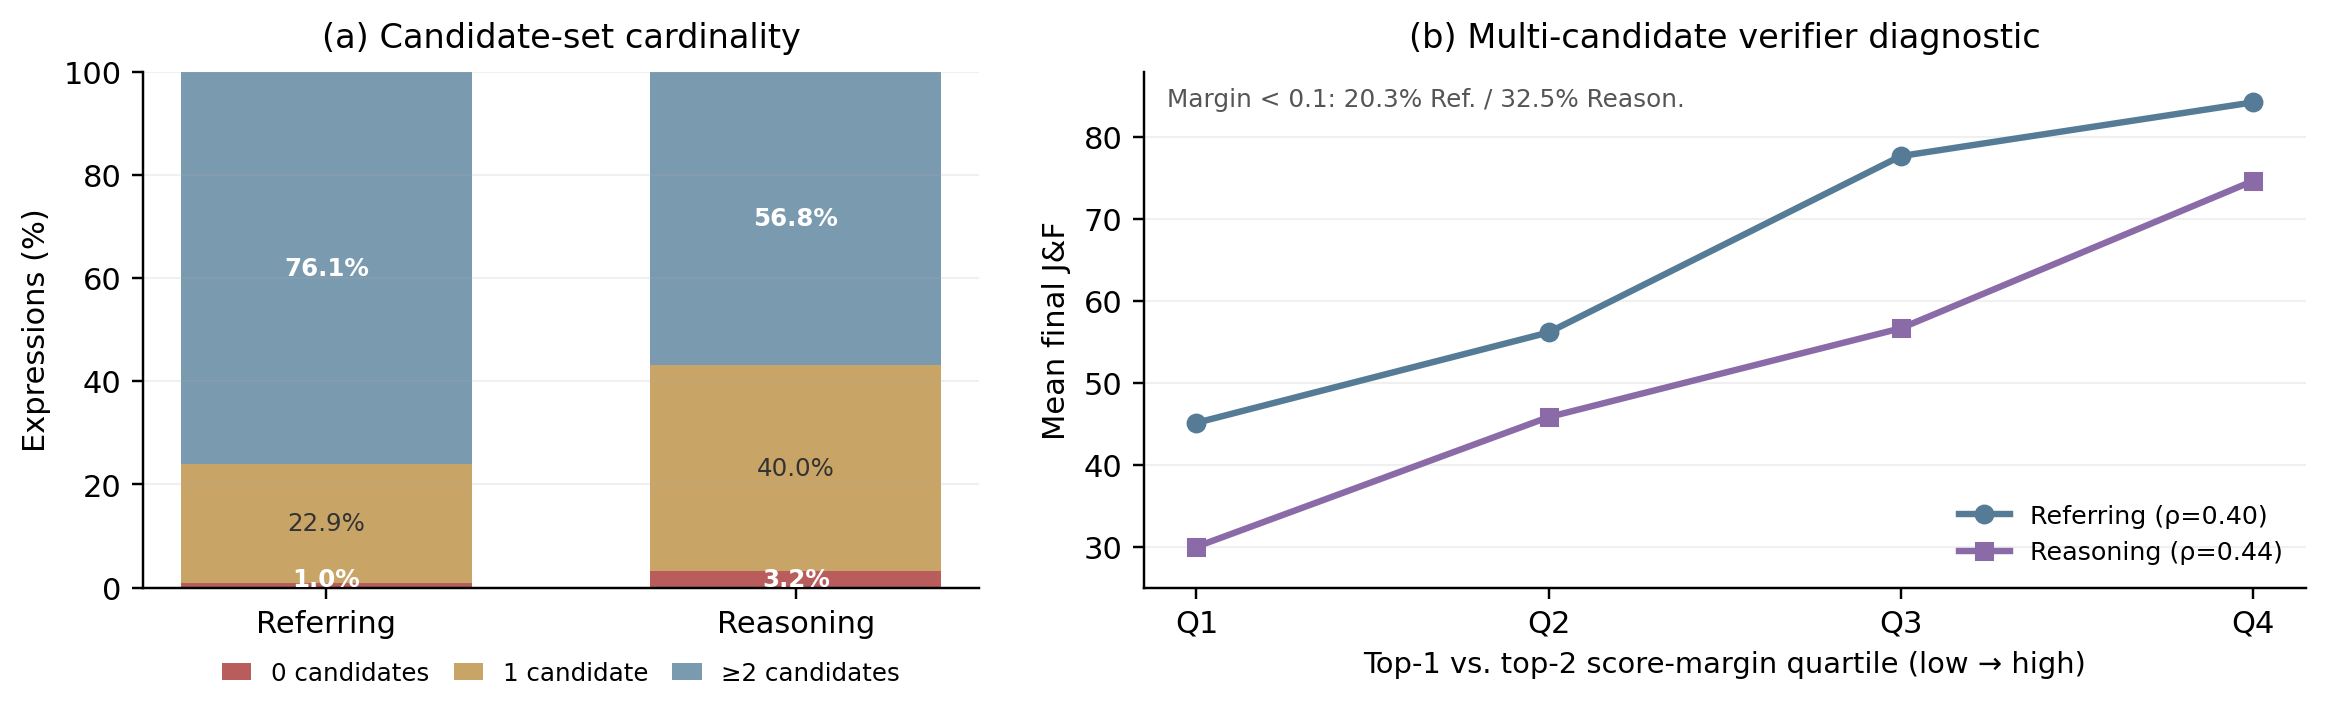
\includegraphics[width=0.91\textwidth]{figures/revos_fullval_diagnostic.png}
  \caption{Post-hoc diagnostic on the completed ReVOS validation run. Left: retained candidate-set cardinality for the official referring and reasoning partitions. Right: among expressions with at least two scored candidates, final $\mathcal{J}\&\mathcal{F}$ as a function of the top-1--top-2 verifier score-margin quartile. The association is descriptive and does not isolate candidate quality from semantic ranking difficulty.}
  \label{fig:revos_fullval_diag}
\end{figure*}
\paragraph{Q2: Is candidate recall a measurable bottleneck?}
For an expression $q$, let the oracle candidate overlap be
\begin{equation}
J^{\star}(q)=\max_{\tau_i\in\mathcal{C}(q)} J(\tau_i,Y_q),
\end{equation}
and define candidate recall as $\mathrm{Recall}_{\eta}=\Pr[J^{\star}\geq\eta]$. These quantities characterize the best segmentation available to the verifier before any semantic ranking decision is made. If $J^{\star}$ is low, no downstream verifier can recover a high-quality mask from the retained candidate set.

We use stored \emph{training-side} candidate sets to isolate the effect of widening SAM3 search while keeping the downstream candidate budget fixed. On Ref-Youtube-VOS train, the original top-7 cache contains 12,580 expressions with mean $J^{\star}=77.17$ and Recall@0.5=87.91\%. Re-running low-recall cases with recall-24/keep-7 and overlaying the recovered candidates raises the reconstructed mean $J^{\star}$ to 78.20 and Recall@0.5 to 89.22\%, recovering 165 previously sub-threshold expressions. On Ref-DAVIS17 train, the corresponding change is 65.84$\rightarrow$66.44 mean $J^{\star}$ and 72.32\%$\rightarrow$73.06\% Recall@0.5, recovering four examples. Because these statistics come from cached training candidate sets rather than the benchmark validation protocols, we use them strictly as a mechanism diagnostic and not as an end-to-end comparison.

\begin{figure}[t]
  \centering
  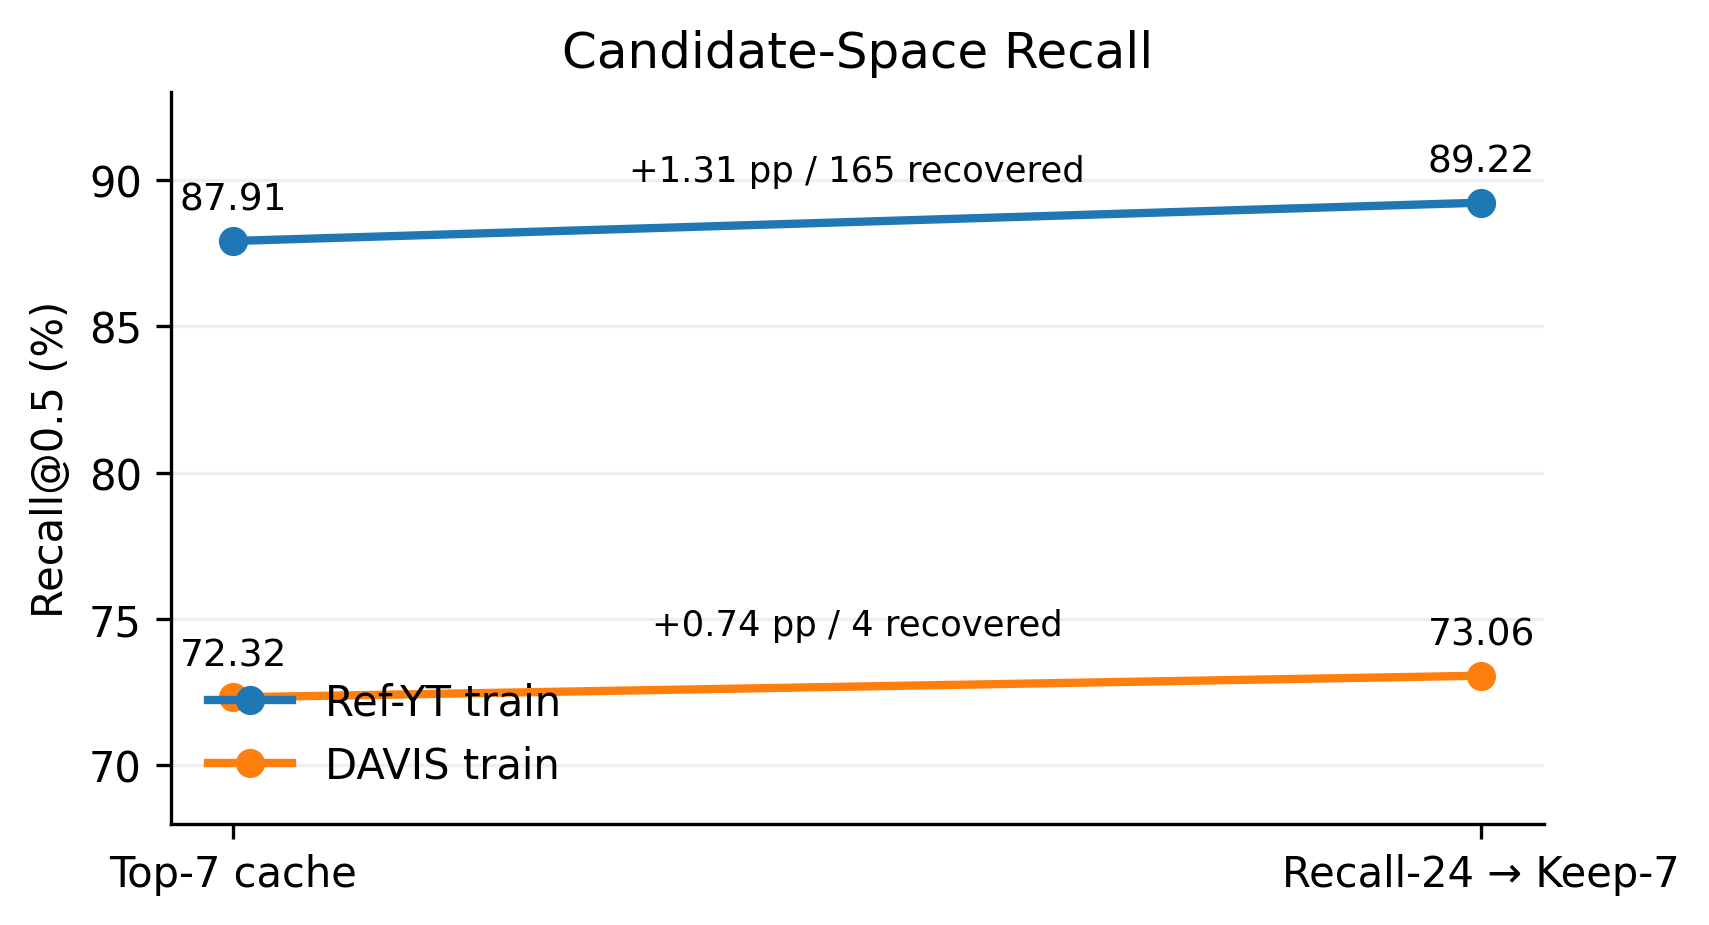
\includegraphics[width=\linewidth]{figures/candidate_space_recall_analysis.png}
  \caption{Training-side candidate-space diagnostic. Expanding SAM3 search from the original top-7 cache to recall-24 followed by keep-7 recovers target hypotheses that were previously below the $J^{\star}=0.5$ threshold.}
  \label{fig:cache_recall}
\end{figure}

Several recovered expressions move from near-zero oracle overlap to above $J^{\star}=0.9$, including cases with small manipulated objects and crowded same-category scenes. The point of this diagnostic is not that a larger search always improves final RVOS performance, but that candidate omission is an irreversible upstream failure: verification can only rank hypotheses that recall has made available.

A direct cross-dataset test of whether SAM3 recall quality explains the different final scores on MeViS, Ref-DAVIS17, Ref-Youtube-VOS, and ReVOS requires candidate statistics extracted under each corresponding inference configuration. Those matched statistics are not available for all four benchmarks in the present study, so we refrain from making a cross-dataset correlation claim and restrict the evidence above to the controlled training-side recall diagnostic.

\paragraph{Q3: Does learned verification improve discrimination once candidates are fixed?}
We isolate the verifier on a fixed MeViS candidate set so that upstream recall is identical before and after verifier training. Figure~\ref{fig:cls_rank_analysis} compares the base Qwen3-VL scorer with the trained candidate verifier. The mean $P(\mathrm{Yes})$ assigned to positive candidates rises from 0.4857 to 0.7685, while the mean probability assigned to negative candidates falls from 0.4558 to 0.1917. More importantly, the within-expression Yes--No logit gap between the strongest positive and strongest negative candidate changes from $-1.3625$ to $4.1788$. The top-1 positive rate improves from 37\% to 78\%, and 47\% of expressions switch from an incorrect top-ranked hypothesis to a positive candidate. Since the candidate set is held fixed, these gains directly measure improved candidate discrimination rather than improved recall.

\begin{figure}[t]
  \centering
  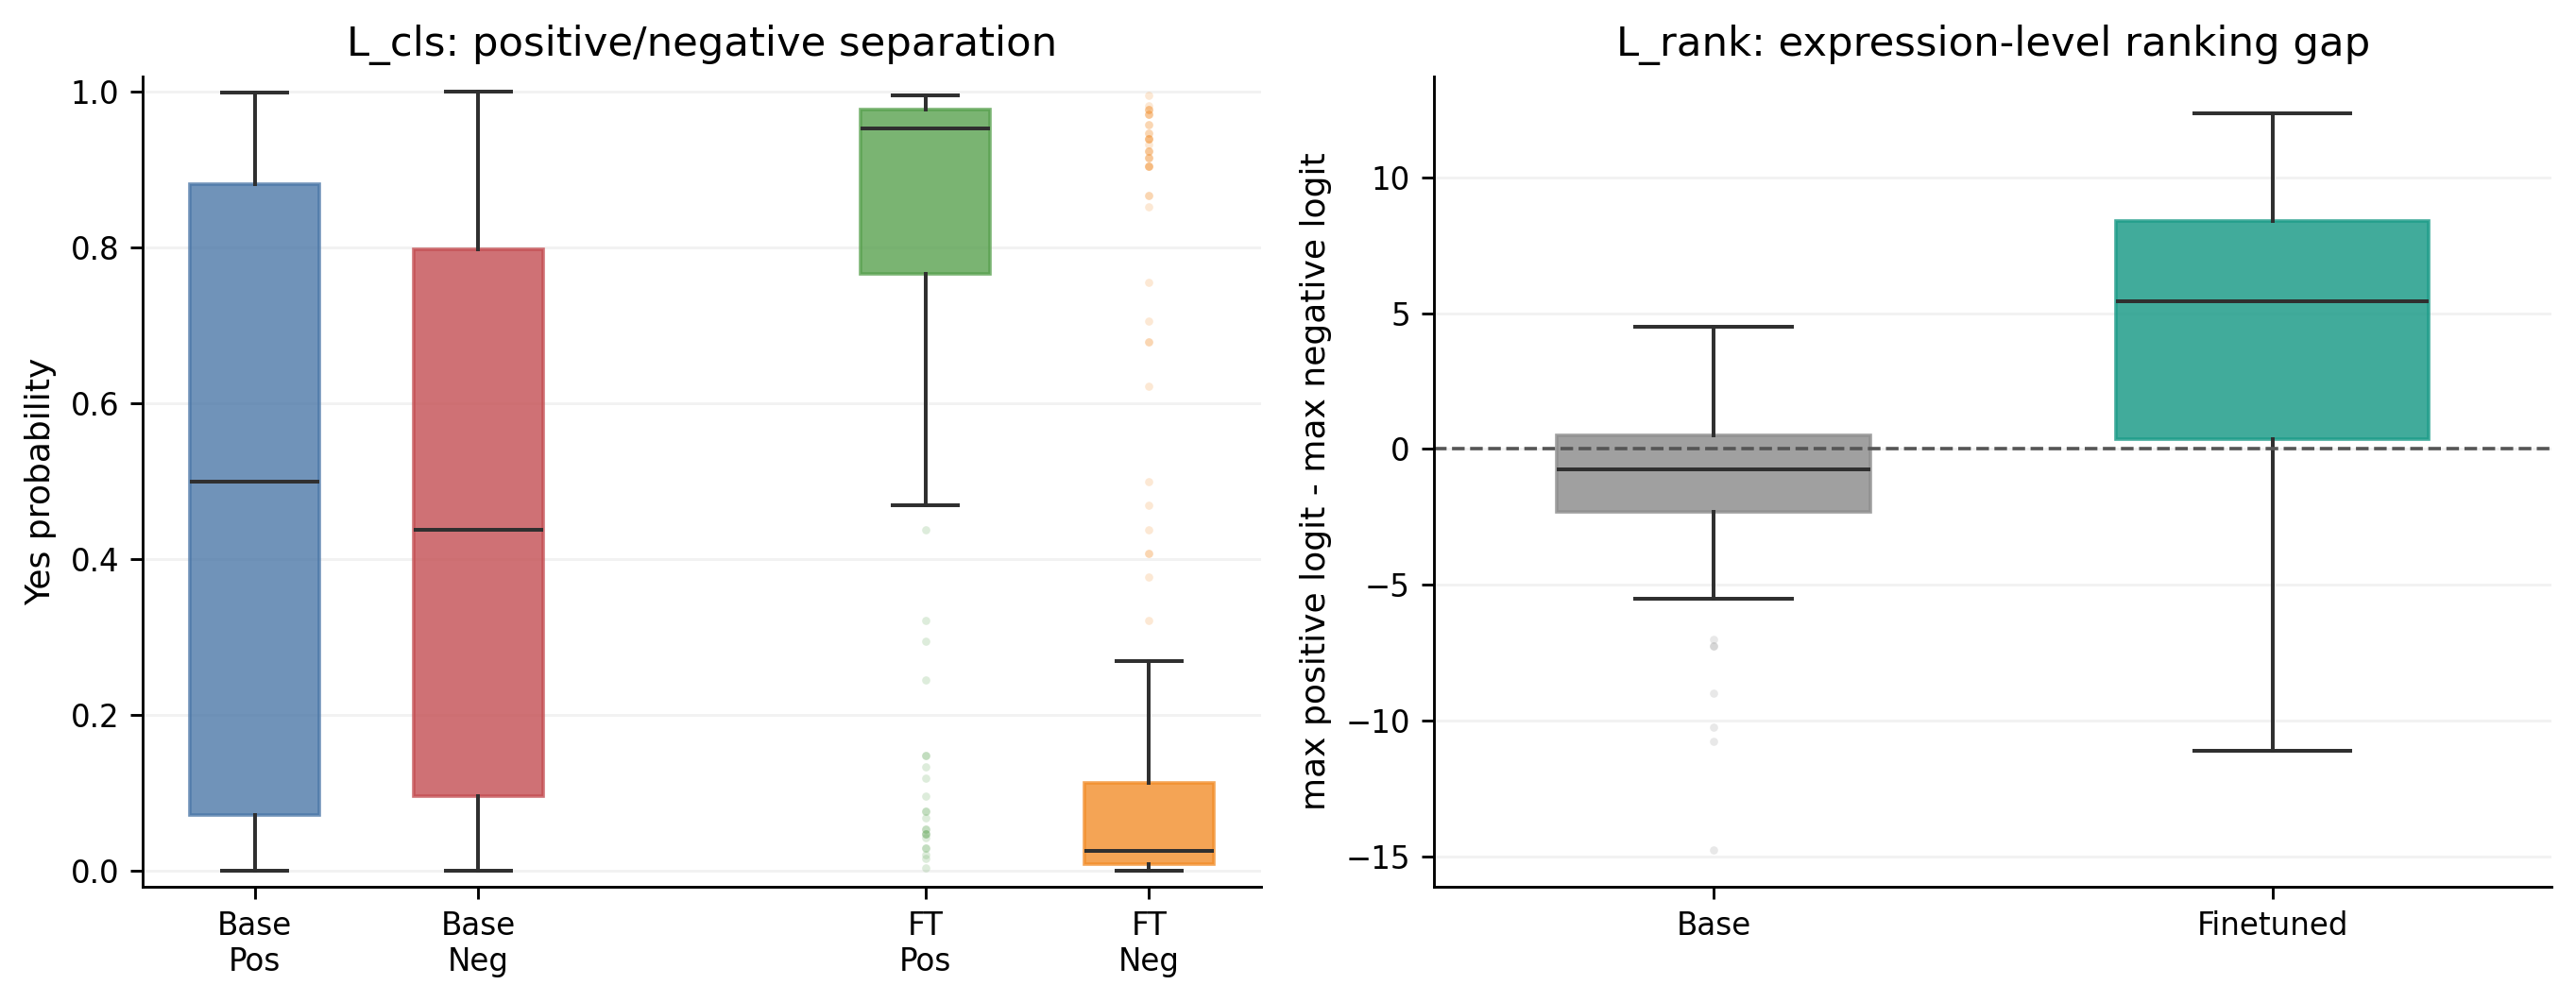
\includegraphics[width=\linewidth]{figures/paper_cls_rank_main.png}
  \caption{Verifier-only analysis on fixed MeViS candidate sets. Left: positive and negative $P(\mathrm{Yes})$ before and after verifier training. Right: the within-expression ranking gap between the strongest positive and strongest negative candidate.}
  \label{fig:cls_rank_analysis}
\end{figure}


\subsection{Real Qualitative Cases}
Figure~\ref{fig:real_qualitative} connects the full-validation diagnostic to four concrete examples. Cases are selected for illustration using candidate count, score margin, and final sequence-level accuracy, followed by visual inspection; they are not a random sample or an additional performance estimate. The referring expressions, recall concepts, candidate scores, and final predictions come from the completed ReVOS run. Since non-selected candidate masks were not archived per expression, we replay only frozen SAM3-DMS recall with the recorded concept and recall-24/keep-7 settings. The retained candidate IDs agree in all four examples, and the selected tube is pixel-identical to the archived output on all frames of cases A--C. The replay candidate column is explicitly distinguished from the historical scores and predictions.

Case A distinguishes one cat among five same-category hypotheses, with a score margin of 0.671 and final $\mathcal{J}\&\mathcal{F}=98.51$. Case B illustrates a temporal query about which joystick is held at the end of the video: the concept \emph{joystick} admits two hypotheses, while the full expression specifies the intended referent. Its margin is 0.905 and final $\mathcal{J}\&\mathcal{F}=97.98$. This is an illustrative success rather than an ablation establishing that a particular language clause caused the decision.

Case C exposes a different behavior: three cat hypotheses receive high scores, but the top-two margin is only 0.014 and the selected object is disjoint from the target, giving $\mathcal{J}\&\mathcal{F}=0$. In the independently recorded recall replay, an alternative candidate reaches $\mathcal{J}\&\mathcal{F}=93.86$, making this a useful example for inspecting candidate selection rather than interpreting a high absolute Yes probability as correctness. The replay does not establish pixel identity for every unselected historical candidate. Finally, case D yields no candidate for the recorded concept \emph{bull}, leaving an empty final prediction despite a visible annotated target. It localizes the failure to the Ground--Recall interface; without a controlled prompt intervention, it does not distinguish lexical grounding from the segmenter's response to the concept.

\begin{figure*}[t]
  \centering
  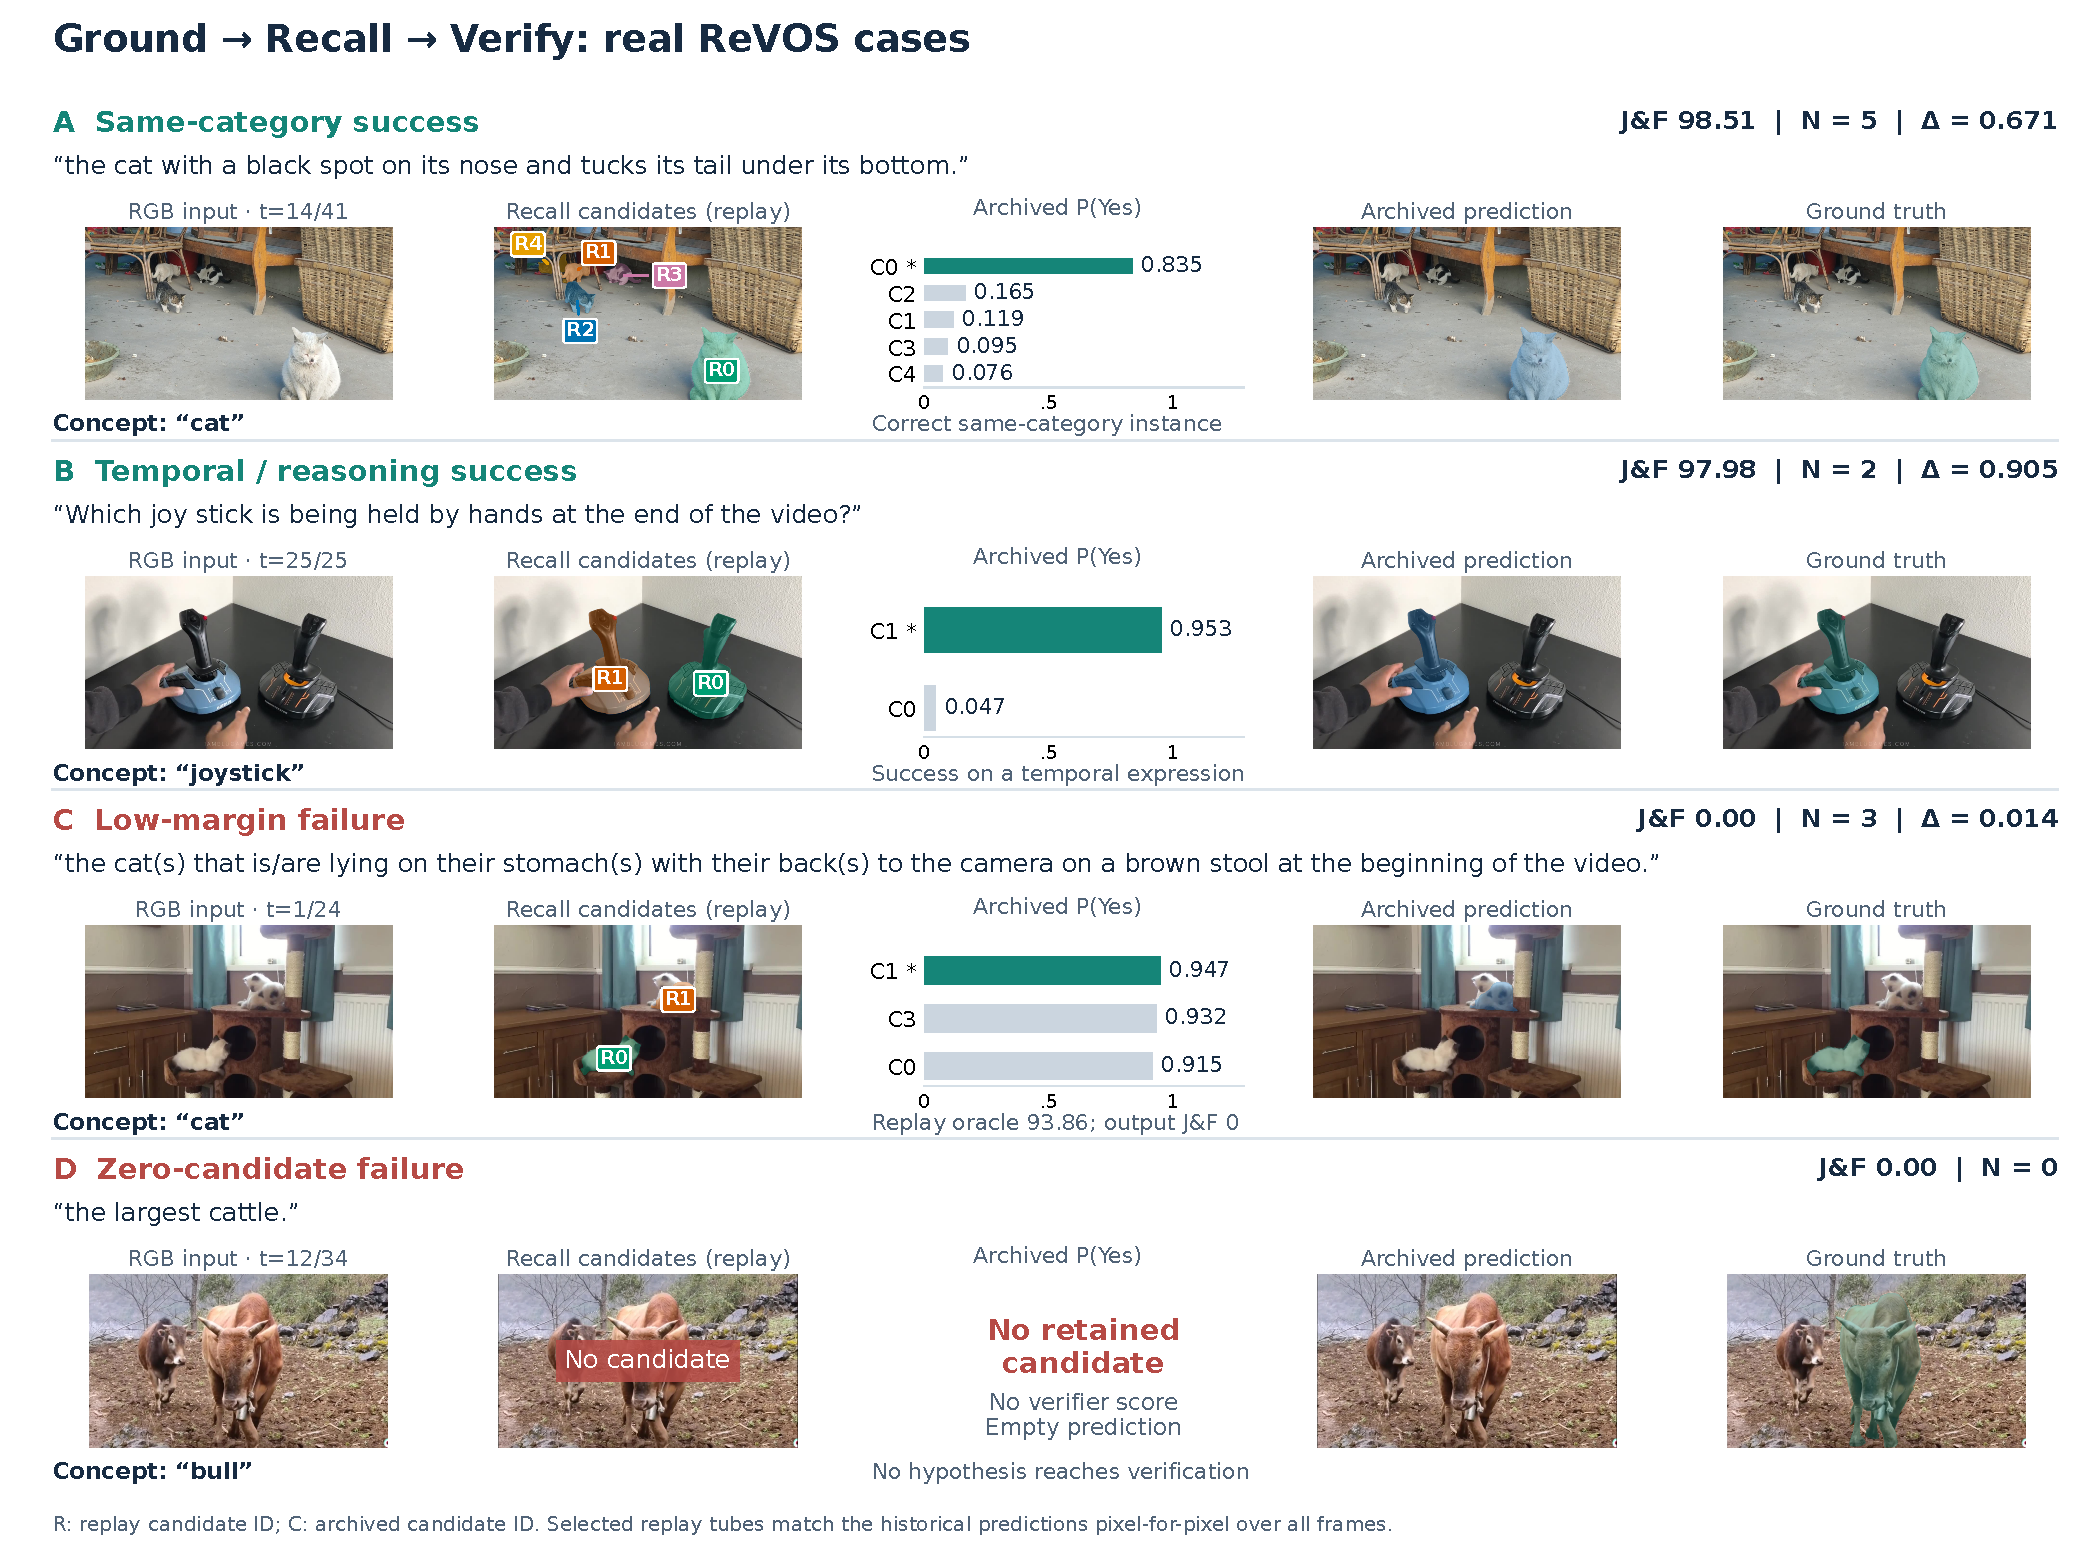
\includegraphics[width=\textwidth]{figures/revos_qualitative_pipeline.pdf}
  \caption{\textbf{Real Ground--Recall--Verify examples on ReVOS.} A: same-category success. B: temporal/reasoning success. C: low-margin selection failure. D: no retained candidate. Each row shows the original expression, recorded recall concept, one RGB frame, replayed SAM3 candidates, archived verifier scores, archived final prediction (blue), and GT (green). $N$ counts scored candidates and $\Delta$ is the top-1--top-2 score gap. $\mathcal{J}\&\mathcal{F}$ is measured over the full video, not only the displayed frame. R denotes a replay candidate ID and C an archived score ID; the selected replay tube matches the archived mask in every frame of A--C. Non-selected replay masks are not claimed to be archived verifier inputs. Only candidates visible at the displayed time have spatial overlays. The overlays are editorial visualizations.}
  \label{fig:real_qualitative}
\end{figure*}

\subsection{Discussion and Limitations}
\paragraph{An explicit error decomposition.}
The candidate-space formulation exposes three failure modes that are entangled in direct language-to-mask systems. \textbf{Grounding failures} occur when the generated recall concept is not sufficiently tied to the referred visual evidence. \textbf{Recall failures} occur when the concept is plausible but SAM3 fails to place a sufficiently accurate target tube in the retained candidate set. \textbf{Verification failures} occur when a good target tube is present but a distractor receives a higher semantic score. This decomposition separates whether the target was \emph{made available} to the verifier from whether it was \emph{chosen correctly} once available.

\paragraph{Prompt-sensitive recall.}
The recall concept is not merely an intermediate textual description; it controls which object hypotheses SAM3 exposes. A semantically plausible but visually misgrounded, over-specific, or lexically mismatched concept can remove the target before verification begins. The training-side candidate diagnostic in Fig.~\ref{fig:cache_recall} demonstrates the resulting upper-bound effect, but it does not by itself establish a cross-dataset correlation between recall quality and final accuracy. Establishing that stronger claim requires the matched validation-side candidate statistics described above. This distinction is important: we use candidate-space analysis to identify a plausible bottleneck, not to retroactively explain every benchmark difference.

\paragraph{Stage decoupling and future coupling.}
Grounding/recall and verification are deliberately modular, but their learned components are optimized with separate objectives. Candidate quality at the intermediate SAM3 interface therefore does not directly supervise the grounder. A natural extension is to introduce candidate-aware grounding objectives, share lightweight expression-conditioned adapters, or alternate the stages so that difficult verifier cases become informative grounding examples. Such coupling may preserve the interpretability of an explicit candidate space while allowing downstream candidate quality to shape upstream concept formation.

\paragraph{Other limitations.}
The multi-stage pipeline is more expensive than a compact end-to-end segmenter because multiple hypotheses must be generated and evaluated. Recall remains difficult for small, heavily occluded, briefly visible, or unusually named objects, while the full-validation ReVOS result shows that reasoning-oriented expressions remain challenging for the compact 4B verifier. These limitations motivate adaptive candidate budgets, more prompt-robust concept formation, and more efficient track-level reasoning.
